\documentclass[a4paper,11pt]{article}
\input{/home/tof/Documents/Cozy/latex-include/preambule_lua.tex}
\newcommand{\showprof}{show them}  % comment this line if you don't want to see todo environment
\fancyhead[L]{Publier une page web}
\newdate{madate}{10}{09}{2020}
%\fancyhead[R]{\displaydate{madate}} %\today
\fancyhead[R]{Seconde - SNT}
%\fancyhead[R]{Première - NSI}
%\fancyhead[R]{Terminale - NSI}
\fancyfoot[L]{~\\Christophe Viroulaud}
\AtEndDocument{\label{lastpage}}
\fancyfoot[C]{\textbf{Page \thepage/\pageref{lastpage}}}
\fancyfoot[R]{\includegraphics[width=2cm,align=t]{/home/tof/Documents/Cozy/latex-include/cc.png}}

\begin{document}
\begin{Form}
\section{Problématique}
Le (joli) site web que nous avons crée n'est pas accessible par une autre personne. La dernière étape à réaliser est de le \textbf{publier}.
\begin{center}
\shadowbox{\parbox{10cm}{\centering Comment rendre un site accessible sur le web?}}
\end{center}
\section{Principe}
Le réseau \emph{internet} (figure \ref{reseau}) relie tous les ordinateurs entre eux.
\begin{center}
\centering
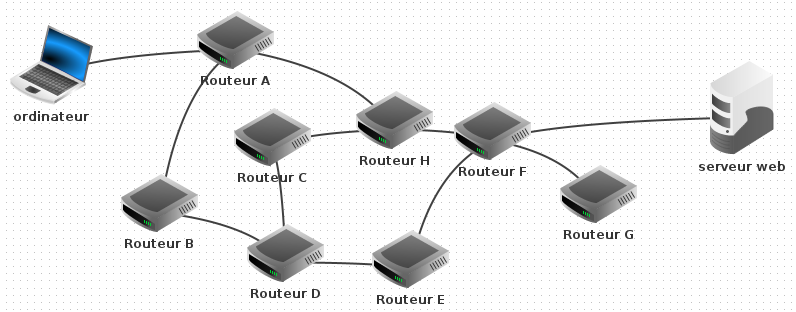
\includegraphics[width=12cm]{ressources/serveur-web.png}
\captionof{figure}{Réseau internet}
\label{reseau}
\end{center}
Les \textbf{serveurs web} ont un rôle particulier. Ces machines stockent les fichiers des sites internet. Quand un visiteur désire consulter une page web elle demande la page au serveur. Ce-dernier lui renvoie le contenu de la page demandée (figure \ref{reseau}).\\
Le cours \emph{DNS} apporte davantage de précisions sur cet échange.
\begin{center}
\centering
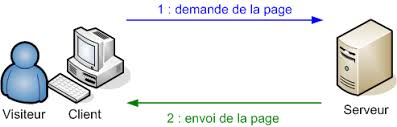
\includegraphics[width=8cm]{ressources/http.jpeg}
\captionof{figure}{Consulter un site}
\label{consult}
\end{center}

\section{Publication}
Pour publier un site il faut donc le déposer sur un serveur web. Les fournisseurs d'accès internet proposent généralement la possibilité de créer une \emph{page personnelle}.
\begin{activite}
\begin{enumerate}
\item Renommer le dossier du site web: \emph{mon-nom-de-famille}. Ne pas mettre d'espace ni d'accent.
\item Donner le dossier au professeur.
\item Le site sera disponible à l'adresse 
\begin{center}
\url{https://cviroulaud.github.io/sites/mon-nom-de-famille}
\end{center}
L'exemple du professeur:
\begin{center}
\url{https://cviroulaud.github.io/sites/viroulaud}
\end{center}
\end{enumerate}
\end{activite}
\end{Form}
\end{document}